% !TEX root=../pldi2019.tex


\section{Semantics}



\subsection{Layered semantics}
\label{sec:normalise}
\label{sec:drive}

Stepping from one task to another using the sequence construct $\Then$ is done by the system itself,
not by the user.
We will call this an \emph{internal step} or \emph{system step}.\footnote{
  This implies there will also be an \emph{external step} or \emph{user step} performed on users' request.
  This is indeed the case and we will discuss it in \autoref{sec:external-step}.
}
As there is no explicit user input needed to perform an internal step,
we cannot use our event handling semantics $\handle{h}$,
described in \autoref{sec:handling},
to specify stepping from one task to the next (calculated) one.
Also,
using our evaluation semantics to do so,
would pollute the semantics our our host language with rules specific for the task layer.

Therefore we introduce another semantic relation which we will call \emph{normalisation}.
When considering our semantic relations as a hierarchy,
normalisation conceptually lies \emph{between} evaluation and handling.
Normalisation will make use of evaluation of our underlying host language and,
as we will see later on,
handling will make use of normalisation
and the functions $\Value(t)$ and $\Failing(t)$ from sections \autoref{sec:value} and \autoref{sec:failing}.

Graphically,
we now have the following semantic functions shown in \autoref{fig:semantic-functions}.
Note that the double down arrow $\stride$ \emph{uses} the single down arrow $\evaluate$,
a convention we will use again later in this text.

\begin{figure}[h]
  \centering
  \includegraphics[width=0.7\columnwidth,page=4]{figures/drawings-crop.pdf}
  \caption{
    Semantic functions defined in this report and their relation.
  }
  \label{fig:semantic-functions}
\end{figure}
\todo{Fix figure to contain all observation and new striding}

As evaluation,
normalisation is a \emph{big step} semantics.
We write \refrule{RelationN} to describe that
task $t$ normalises to task $t'$.
Note that, as handling,
normalisation \emph{only acts upon tasks}.
It is a semantic relation that lives \emph{on the task level}.
We can think of normalisation as a \enquote{medium step} semantics,
normalising tasks $t$ as much as possible,
till the moment it needs an event to continue.
For editors and the failing task normalisation is simple.
\refrule{S-Edit} \refrule{S-Fill} \refrule{S-Fail}
In the next subsection we will introduce rules to normalise a task sequence.

To ensure tasks are ready to process the next event,
we need to normalise after each use of the handling semantics.
Instead of adding normalisation to every handling rule,
we introduce a fourth semantic relation to deal with this.
The drive relation $\RelationD$ simply passes the event $h$ to the handle semantics
and normalises the task afterwards.
\refrule{D-Handle}
Note that again,
the double arrow $\drive{h}$ uses the single arrow $\handle{h}$.



\subsection{Evaluation semantics}
\label{sec:evaluation}

To express evaluation,
we use the big step semantics of our host language.
Turning an expression $e$ into a value $v$ is denoted by $e \evaluate v$.
The rules to evaluate expressions $e$ do not differ from standard work.

Regarding our base language, lambda abstractions are values, as are all constants.
Each \emph{pretask} $p$ we will encounter in the upcoming sections,
will be accompanied by a corresponding \emph{task} $t$.
Tasks are also values with respect to evaluation.
This means pretasks will be eagerly evaluated to tasks by the relation $\evaluate$.\footnote{
  The same applies to pairs,
  which we will add to our host language in \autoref{sec:pairing}.
}
This suggestion by \textcite[p. 323]{books/Harper16PFPL}
makes it easier to reason about data constructors.

\begin{figure}
  \small
  \begin{mathpar}
    \boxed{\RelationE} \\
    \userule{E-Edit} \quad
    \userule{E-Fill} \quad
    \userule{E-Update} \\
    \userule{E-Then} \quad
    \userule{E-Next} \\
    \userule{E-And} \\
    \userule{E-Or} \quad
    \userule{E-Xor} \\
    \userule{E-Appoint} \quad
    \userule{E-Fail} \\
  \end{mathpar}
  \caption{Evaluation semantics} \label{fig:evaluation-semantics}
\end{figure}


\paragraph{Evaluating pretasks to tasks}
\label{sec:tasks-vs-pretasks}

Till now, syntactically we only talking about \emph{pretasks}.
Now the time has come to talk about \emph{real} tasks!
Well, about \emph{syntactically real} tasks.

So what is the difference with pretasks?
The subtle change from $\Edit e$ to $\Edit v$ in the valued editor.
That is, an editor with an arbitrary (although well typed) expression $e$,
versus an editor with an (evaluated) value $v$.
Coming from one to the other is done by the evaluation relation we introduced in \autoref{sec:evaluation}.

There are two rules we need to add for this semantic arrow to accomplish this:
one for valued and one for unvalued editors.
\refrule{E-Edit} \refrule{E-Fill}
Rule \refrule{E-Edit} uses the big step semantics from our base language ($\evaluate$)
to evaluate the wrapped expression $e$ to a value $v$ and rewraps it in an editor.
Rule \refrule{E-Fill} has nothing to evaluate and just keeps the unvalued editor as is.

Summarising, pretask $p$ allow us to syntactically write down arbitrary expressions inside a valued editor,
or any other pretask we will define in the future.
Tasks $t$ are pretasks \emph{after evaluation} using the relation $\evaluate$.
With other words:
\begin{itemize}
  \item
    Pretasks $p$ are task expressions.
  \item
    Tasks $t$ are a syntactical subset of pretasks $p$.
    They are values with respect to evaluation, i.e. the relation $\evaluate$.
\end{itemize}


\subsection{Two principles of stepping}
\label{sec:normalise-sequence}

Above rules imply that we have three cases when normalising a sequence.
First,
it could be the case that the left hand side does not have a value after normalisation.
This means we cannot pass a value to the right hand side
and thus we cannot make the step.
\refrule{S-ThenStay}

Second,
the normalised left hand side has a value,
but when evaluating the right hand side,
it leads to a failing task.
We do not allow stepping to a failing task
and thus we also cannot make a step.
\refrule{S-ThenFail}
Note we use the evaluation semantics of our host language
to evaluate the function application $e_2\ v_1$ to a new task $t_2$.

Third,
the normalised left hand side has a value,
and the evaluated right hand side is a succeeding task.
Now we can make a step!
\refrule{S-ThenCont}
Note we normalise $t_2$ first before yielding our result.

The sequence construct itself does not handle any user input.
The left hand side however,
can be an interactive task, such as an editor.
To reach this encapsulated interactive task,
$\Then$ needs to pass inputs to the left.
\refrule{H-PassThen}

Almost there!
We did not extend the functions $\Failing(t)$ and $\Value(t)$ for our new sequencing construct $\Then$.
Intuitively,
when we have a task $\Fail \Then e_2$ we are stuck.
As in the case of just the task $\Fail$,
users can send any event,
but nothing will ever happen.
$\Fail$ will never have a value
and therefore $\Then$ will never make a step to $e_2$.\footnote{
  This is a property called \emph{left absorption},
  which tells us something about the interaction between $\Fail$ and $\Then$.
  See also \autoref{sec:monad-laws}.
}
If the left hand side of $\Then$ is any other task,
all will be well.
Thus,
a sequence $t_1 \Then e_2$ is succeeding iff its left hand side $t_1$ is succeeding.

The question remains what value we have to associate to a task sequence.
The answer is: none!
Imagine the task $t := \Edit \str{Hello} \Then \lambda s.\allowbreak\Edit (\Length s)$,
where a user entered a string and our task gives the length of the string as the result.
Recall the definition of $\Value(t)$ from \autoref{sec:value}.
The value of the left hand side of $t$ is the string $\str{Hello}$.
After stepping to the right hand side,
the value of $t$ should be $\Value(\Edit (\Length\str{Hello})) = \Value(\Edit 5) = 5$.
This means the type of the value \emph{changed} after taking the step.
\todo{Elaborate more about why this is not desirable.}
Therefore we define that a sequence of tasks \emph{does not} have a value.\footnote{
  We could choose that the value of a sequence equals the value of the left hand side.
  This will have fatal consequences for our stepping semantics however.
}


\subsection{Observation semantics}


\paragraph{Task value}

\paragraph{Inputs}

\paragraph{Failing}

When an expression fails, it can not be normalised and there is no possible
input that it will handle. The function $\Failing$ determines this property.

\paragraph{User Interface }



\subsection{Normalisation semantics}

\begin{figure}
  \small

  \begin{mathpar}
    \boxed{\RelationS}
  \end{mathpar}

  \paragraph{Step}
  \begin{mathpar}
    \userule{S-ThenStay} \\
    \userule{S-ThenFail} \\
    \userule{S-ThenCont}
  \end{mathpar}

  \paragraph{Choose}
  \begin{mathpar}
    \userule{S-OrLeft} \\
    \userule{S-OrRight} \\
    \userule{S-OrNone}
  \end{mathpar}

  \paragraph{Ready}
  \begin{mathpar}
    \userule{S-Edit} \quad \userule{S-Fill} \qquad \userule{S-Update} \\
    \userule{S-Fail} \quad \userule{S-Xor}
  \end{mathpar}

  \paragraph{Congruence}
  \begin{mathpar}
    \userule{S-Next} \quad
    \userule{S-And} \\
    \userule{S-Appoint}
    % \userule{S-Eval}
  \end{mathpar}

  \caption{Striding semantics} \label{fig:normalisation-semantics}
\end{figure}

\begin{figure}
  \small
  \begin{mathpar}
    \boxed{\RelationN} \\
    \userule{N-Done} \\
    \userule{N-Stride}
  \end{mathpar}
  \caption{Normalisation semantics} \label{fig:memory-semantics}
\end{figure}


\subsection{Handling inputs}
\label{sec:handling}

\begin{figure}
  \usemacro{G-Inputs}
  \caption{Input grammar} \label{fig:input-grammar}
\end{figure}

To change values in an editor,
we should interact with the user by some kind of interface.
In a graphical setting,
we can present the user an input box.
The user can then change and clear values continuously.
In a text oriented world,
we can print out the current value of an editor
and prompt the user for a new value
or a command to empty the editor.

To abstract away from the user interface,
we introduce an event system.
It does not matter how these events are sent to the application.
This can be by pushing a button,
entering text in an input box,
committing some text on a command line,
sending it over a web socket,
etc.

In a previous attempt to build a semantics for \TOP,
\textcite{theses/radboud/VinterHviid18} also used the notion of events.
However, \citeauthor{theses/radboud/VinterHviid18} made events part of the task layer.
This means the programmer has access to events using a \texttt{getEvent} function call.

In this work,
we deviate from above idea.
We use labeled transitions in the same way as \textcite{school/maktoberdorf/PeytonJones01},
who gives denotational semantics to the Haskell \IO monad.
Therefore events live on the \emph{semantic level} only
and they are \emph{not} accessible from within our language.

We define a new syntactic category of \emph{events} $h$.
For now, they only contain \emph{actions} $a$.
We will introduce more events and actions in later sections.

As we already discussed before,
there are three actions that can be handled by editors:
\begin{enumerate*}
  \item filling in an unvalued editor;
  \item changing the value; or
  \item clearing the value.
\end{enumerate*}
We choose to merge the first two, filling and changing, into one action.
The value of an editor, empty or not, can be changed to a value $v$ by just sending the value as an action.
To empty a valued editor, we send the $\Empty$(mpty) action.

Handling inputs is done by a new semantic relation.
This small step relation takes a task $t$ and an event $h$ which results in a new task $t'$.
We write $\RelationH$
Formalising the states and transitions shown in \autoref{fig:editor-state},
we need three rules to describe editors.
\refrule{H-Change} \refrule{H-Empty} \refrule{H-Fill}
Note that the conditions to the right of the rules take care of typing.
Only when the entered value $v'$ has the same type $\beta$ as the original value $v$ we can change a valued editor.
In case of an unvalued editor,
the entered value $v'$ needs to have the same type as the type annotation $\beta$.
These conditions make sure the type of the entered value and the type of the editor are always the same.

\begin{figure}
  \small

  \begin{mathpar}
    \boxed{\RelationH}
  \end{mathpar}

  \paragraph{Editing}
  \begin{mathpar}
    \userule{H-Change} \quad
    \userule{H-Empty} \\
    \userule{H-Fill} \quad
    \userule{H-Update}
  \end{mathpar}

  \paragraph{Continuing}
  \begin{mathpar}
    \userule{H-PickLeft}\\
    \userule{H-PickRight} \\
    \userule{H-Next}
  \end{mathpar}

  \paragraph{Passing}
  \begin{mathpar}
    \userule{H-PassThen} \quad \userule{H-PassNext} \\
    \userule{H-FirstAnd} \quad \userule{H-SecondAnd} \\
    \userule{H-FirstOr}  \quad \userule{H-SecondOr}\\
    \userule{H-Assign}
  \end{mathpar}

  \caption{Handling semantics} \label{fig:handling-semantics}
\end{figure}


\paragraph{Memory}

\paragraph{Driving}

\begin{figure}
  \small
  \begin{mathpar}
    \boxed{\RelationD} \\
    \userule{D-Handle}
  \end{mathpar}
  \caption{Driving semantics} \label{fig:driving-semantics}
\end{figure}




\todo{Merge observations in one big table over two columns at top of page?}

\begin{figure}
  \small
  \usemacro{O-Value}
  \caption{Values} \label{fig:observation-value}
\end{figure}

\begin{figure}
  \small
  \usemacro{O-Inputs}
  \caption{Inputs} \label{fig:observation-value}
\end{figure}

\begin{figure}
  \small
  \usemacro{O-Failing}
  \caption{Failing} \label{fig:observation-failing}
\end{figure}

\begin{figure}
  \small
  \usemacro{O-Watching}
  \caption{Watching} \label{fig:observation-watching}
\end{figure}
